% !TEX TS-program = pdflatex
% !TEX root = ../ArsClassica.tex

%************************************************
\chapter{Matheuristic Methods}
\label{chp:4-Matheuristics}
%************************************************
Given that the \textsc{CPLEX}'s heuristics are not specialized for our problem, we apply the heuristic in the model writing. In this way the model that we’ll give to \textsc{CPLEX} should be theoretically easier to solve.

\section{Hard Fixing}
The first matheuristic algorithm that we have implemented relied on the hard variable-fixing approach. The main idea is to use a \textit{black-box} solver which receives the input data and quickly generates a first solution. Once the initial solution has been found, some of its variables are fixed and then the method is iteratively reapplied on the restricted problem resulting from fixing: the \textit{black-box} solver is called again, a new target solution is found, some of its variables are fixed, and so on. The choice of which variables have to be fixed is arbitrary, so they are chosen with uniform probability.\\
Each time, before applying the \textsc{CPLEX} solver, the algorithm fixes some variables that are equal to 1 in the last solution obtained; an important parameter that influences the performances of the \textsc{CPLEX} solver is the number of edges that have been fixed in each loop. If the number of fixed edges is high, \textsc{CPLEX} will find a solution more quickly. On the other hand, if the number of fixed edges decreases, \textsc{CPLEX} is more free to find better improvements. \\
We chose to fix all the arcs with probability 0.5. 
Using the hard fixing technique, and in general fixing some variables, \textsc{CPLEX} becomes faster because the number of free variables decreases for three reasons: 
\begin{enumerate}
\item some of them are fixed
\item because we "delete" all the arcs exiting from a node which already has an exiting arc
\item because we "delete" all the arcs crossing those already fixed.
\end{enumerate}
We discovered that in the first \textsc{CPLEX} solutions very often appears the "star" solution, see Figure \ref{img:relax1}. The "star" is a shape of routing cables in which all the turbines are directly connected to the substation; in almost all the instances it is not a good solution because of the long cables. This fact can be a problem for the Hard Fixing technique because it is most likely to choose fixed cables far away from the optimal solution. To avoid this situation we have defined a \textit{timestart}: at its first execution, \textsc{CPLEX} runs for \textit{timestart} seconds searching a good starting solution, then it starts the real Hard Fixing method until the \textit{timelimit} expires. 

\subsection{RINS Hard Fixing}
This solution is like the classic Hard Fixing solution with the added condition that when we have to choose a fixed edge, that edge must be present in the actual best solution. Then all the probabilistic mechanisms do not change. This is something like "doing hard fixing over the RINS condition". 


\section{Local Branching (Soft Fixing)}
Given a solution $y^{REF}$, this method (also called \textit{Soft Fixing}) fixes at least a percentage of the arcs of that solution, and repeats the execution searching the best choice for the others, proposed by [\cite{fischetti2003local}]. A critical issue of variable fixing methods is related to the choice of the variables to be fixed at each step and wrong choices are typically difficult to detect. In this sense, the purpose of the soft fixing is to fix a relevant number of variables without losing the possibility of finding feasible solutions.\\
A possible implementation is, given the solution $y^{REF}$ represented by an array of zeros and ones, given a generic solution $y$ and given a constant $K$:
\[
	\sum_{(i,j):y^{REF}_{ij}=0} y_{ij} + \sum_{(i,j):y^{REF}_{ij}=1} (1-y_{ij}) \quad \leq K
\]
The left-bound side term represents the Hamming distance between $y$ and $y^{REF}$; in practice the constraints allows one to replace only few edges of $y^{REF}$. \\
Then, in our implementation, the algorithm starts producing a heuristic solution $y^{REF}$, adds the local branching constraint to the model and solves it using \textsc{CPLEX}.\\
In our solution we decided to start with $K=3$; each time $K$ is increased by two units until it reaches the maximum of 20: then it restarts from 3. It is important that $K$ changes during the execution to allow \textit{local branching} to explore different solution types. We decided those specific numbers after preliminary tests on some instances.\\
Local Branching avoids a rigid fixing of the variables in favor of a more flexible condition. This allows the new solution to "move" from the older one fixing at each iteration some arcs and moving the other looking quickly for a better solution.\\
This is the symmetric version of this method because it considers equally the 0-1 and the 1-0 flips. 
\newpage
\subsection{Asymmetric Soft Fixing}
In this case we consider only the flips from 1 to 0:
\[
	\sum_{(i,j):y^{REF}_{ij}=1} (1-y_{ij}) \quad \leq K
\]
\[
	\sum_{(i,j):y^{REF}_{ij}=1} y_{ij} \quad \geq \sum_{(i,j):y^{REF}_{ij}=1} 1 - K
\]
\[
	\sum_{(i,j):y^{REF}_{ij}=1} y_{ij} \quad \geq n - 1 - K
\]
This method is more convenient as the asymmetric constraint is sparse, so we decided to use this version for testing. 
\subsection{RINS}
RINS algorithm is a heuristic that explores a neighborhood of the current incumbent solution to try to find a new and improved incumbent.\\
This method use an algorithm called relaxation induced neighborhoods search (RINS), proposed by [\cite{danna2005exploring}]. The algorithm is based on the fact that, during the exploration of the branch-and-cut tree, two solutions are typically at our disposal (the incumbent and the fractional LP solution at the current node). We try to get information about the optimal solution using both of them. In our setting, where we have two feasible solutions, we check the arcs that are selected in both and we add a constraints to the model with the soft fixing strategy a little modified.\\
In the asymmetric case it looks only for the 1 values.
It is possible to realize also the Symmetric RINS that consider also the $0$ values. Anyway, we have discarded this option from the tests because for this specific practice case the selected arcs are more important than the ones not selected.
\section{Results}
The MathEuristic method is intended to find a better solution in less time, without certificating the optimality of the solution. The purpose is to use the \textsc{CPLEX} normal execution inserting and removing some conditions. In the table we can see a Hard and Soft Fixing method with and without using the RINS strategy.\\
The best result that we have obtained is with the Hard Fixing with the RINS strategy but also here the result obtained is quite similar. The performance profile in Figure \ref{img:mathperfprof3} highlights the speed of the Hard Fixing method. \\
If we compare this results with the previous we see that the Matheuristic methods return the best results.

\begin{table}[!h]
\caption{Matheuristic methods results with \textit{timelimit} of 10 minutes}
\begin{tabular}{lllllllll}
\hline
Instance & \multicolumn{2}{l}{\textbf{Hard Fixing}} & \multicolumn{2}{l}{\textbf{\begin{tabular}[c]{@{}l@{}}Hard Fixing\\ RINS\end{tabular}}} & \multicolumn{2}{l}{\textbf{\begin{tabular}[c]{@{}l@{}}Soft Fixing\\ Asymmetric\end{tabular}}} & \multicolumn{2}{l}{\textbf{\begin{tabular}[c]{@{}l@{}}Soft Fixing\\ RINS\end{tabular}}} \\ \hline
         & time              & solution             & time                                     & solution                                     & time                                        & solution                                        & time                                     & solution                                     \\ \hline
data\_01 & 349               & 1.89E+07             & 359                                      & 1.97E+07                                     & 355                                         & 1.89E+07                                        & 478                                      & 1.95E+07                                     \\
data\_02 & 215               & 2.02E+09             & 348                                      & 2.16E+07                                     & 541                                         & 2.15E+07                                        & 364                                      & 2.15E+07                                     \\
data\_03 & 304               & 2.30E+07             & 275                                      & 2.28E+07                                     & 178                                         & 2.28E+07                                        & 319                                      & 2.43E+07                                     \\
data\_04 & 419               & 2.45E+07             & 600                                      & 2.49E+07                                     & 299                                         & 2.53E+07                                        & 279                                      & 2.53E+07                                     \\
data\_05 & 83                & 9.02E+09             & 360                                      & 2.41E+07                                     & 571                                         & 2.42E+07                                        & 357                                      & 2.50E+07                                     \\
data\_06 & 414               & 2.71E+07             & 600                                      & 2.76E+07                                     & 540                                         & 2.49E+07                                        & 484                                      & 2.52E+07                                     \\
data\_07 & 8                 & 8.30E+06             & 234                                      & 8.56E+06                                     & 8                                           & 8.42E+06                                        & 9                                        & 8.23E+06                                     \\
data\_08 & 57                & 8.81E+06             & 236                                      & 8.81E+06                                     & 471                                         & 8.81E+06                                        & 508                                      & 8.81E+06                                     \\
data\_09 & 4                 & 1.01E+07             & 25                                       & 9.88E+06                                     & 6                                           & 1.01E+07                                        & 5                                        & 1.01E+07                                     \\
data\_10 & 528               & 1.03E+07             & 35                                       & 1.03E+07                                     & 11                                          & 1.03E+07                                        & 264                                      & 1.03E+07                                     \\
data\_12 & 2                 & 8.60E+06             & 600                                      & 1.09E+07                                     & 239                                         & 8.60E+06                                        & 56                                       & 8.60E+06                                     \\
data\_13 & 19                & 8.93E+06             & 21                                       & 8.93E+06                                     & 20                                          & 7.40E+06                                        & 23                                       & 8.13E+06                                     \\
data\_14 & 40                & 9.73E+06             & 243                                      & 1.02E+07                                     & 24                                          & 1.01E+07                                        & 186                                      & 1.02E+07                                     \\
data\_15 & 61                & 1.03E+07             & 95                                       & 1.03E+07                                     & 101                                         & 1.03E+07                                        & 232                                      & 1.03E+07                                     \\
data\_16 & 116               & 8.05E+06             & 65                                       & 8.05E+06                                     & 37                                          & 8.05E+06                                        & 363                                      & 8.05E+06                                     \\
data\_17 & 291               & 7.93E+06             & 540                                      & 8.56E+06                                     & 62                                          & 8.56E+06                                        & 90                                       & 8.56E+06                                     \\
data\_18 & 60                & 8.36E+06             & 120                                      & 8.36E+06                                     & 403                                         & 8.36E+06                                        & 404                                      & 8.36E+06                                     \\
data\_19 & 305               & 9.21E+06             & 600                                      & 9.49E+06                                     & 346                                         & 8.35E+06                                        & 358                                      & 1.30E+10                                     \\
data\_20 & 300               & 1.10E+10             & 300                                      & 1.60E+10                                     & 296                                         & 1.50E+10                                        & 275                                      & 3.04E+09                                     \\
data\_21 & 280               & 5.04E+09             & 460                                      & 2.04E+09                                     & 341                                         & 4.04E+09                                        & 600                                      & 3.04E+09                                     \\
data\_26 & 558               & 2.28E+07             & 600                                      & 2.24E+07                                     & 479                                         & 2.24E+07                                        & 600                                      & 2.41E+07                                     \\
data\_27 & 479               & 2.26E+07             & 360                                      & 2.38E+07                                     & 360                                         & 1.54E+07                                        & 600                                      & 1.54E+07                                     \\
data\_28 & 300               & 4.03E+09             & 281                                      & 2.03E+09                                     & 419                                         & 2.70E+07                                        & 356                                      & 3.03E+09                                     \\
data\_29 & 538               & 2.03E+09             & 360                                      & 9.20E+10                                     & 592                                         & 7.03E+09                                        & 360                                      & 9.10E+10                                     \\ \hline
\end{tabular}
\end{table}

\begin{center}
	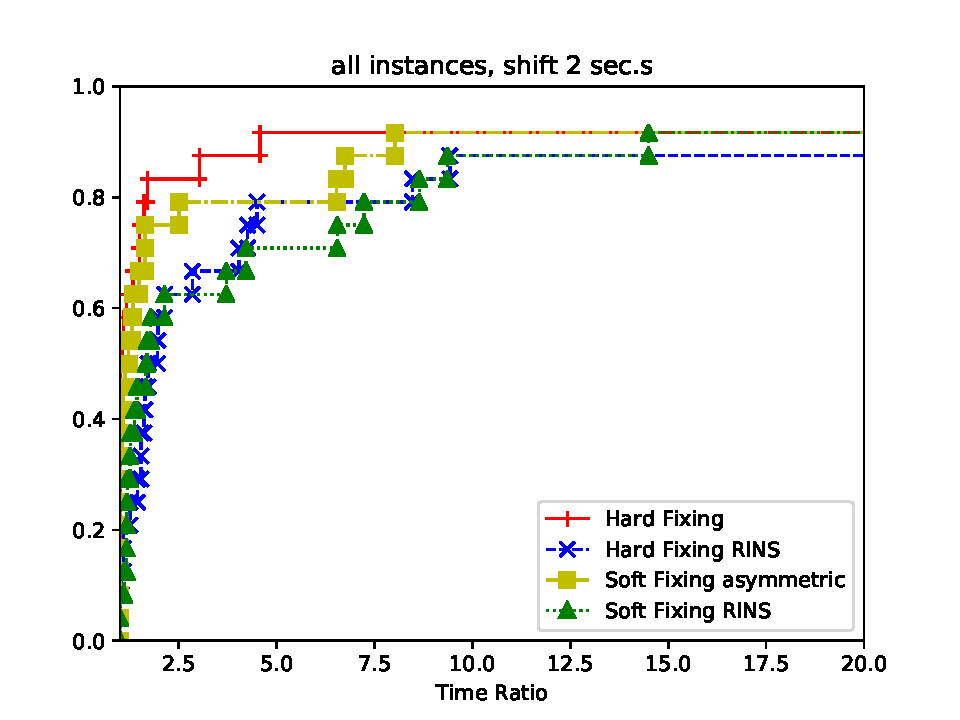
\includegraphics[scale=0.7]{Graphics/Matheuristic.pdf}
	\captionof{figure}{Matheuristics methods performance profile}
	\label{img:mathperfprof3}
\end{center}